% Options for packages loaded elsewhere
\PassOptionsToPackage{unicode}{hyperref}
\PassOptionsToPackage{hyphens}{url}
%
\documentclass[
  ignorenonframetext,
]{beamer}
\usepackage{pgfpages}
\setbeamertemplate{caption}[numbered]
\setbeamertemplate{caption label separator}{: }
\setbeamercolor{caption name}{fg=normal text.fg}
\beamertemplatenavigationsymbolsempty
% Prevent slide breaks in the middle of a paragraph
\widowpenalties 1 10000
\raggedbottom
\setbeamertemplate{part page}{
  \centering
  \begin{beamercolorbox}[sep=16pt,center]{part title}
    \usebeamerfont{part title}\insertpart\par
  \end{beamercolorbox}
}
\setbeamertemplate{section page}{
  \centering
  \begin{beamercolorbox}[sep=12pt,center]{part title}
    \usebeamerfont{section title}\insertsection\par
  \end{beamercolorbox}
}
\setbeamertemplate{subsection page}{
  \centering
  \begin{beamercolorbox}[sep=8pt,center]{part title}
    \usebeamerfont{subsection title}\insertsubsection\par
  \end{beamercolorbox}
}
\AtBeginPart{
  \frame{\partpage}
}
\AtBeginSection{
  \ifbibliography
  \else
    \frame{\sectionpage}
  \fi
}
\AtBeginSubsection{
  \frame{\subsectionpage}
}
\usepackage{lmodern}
\usepackage{amssymb,amsmath}
\usepackage{ifxetex,ifluatex}
\ifnum 0\ifxetex 1\fi\ifluatex 1\fi=0 % if pdftex
  \usepackage[T1]{fontenc}
  \usepackage[utf8]{inputenc}
  \usepackage{textcomp} % provide euro and other symbols
\else % if luatex or xetex
  \usepackage{unicode-math}
  \defaultfontfeatures{Scale=MatchLowercase}
  \defaultfontfeatures[\rmfamily]{Ligatures=TeX,Scale=1}
\fi
% Use upquote if available, for straight quotes in verbatim environments
\IfFileExists{upquote.sty}{\usepackage{upquote}}{}
\IfFileExists{microtype.sty}{% use microtype if available
  \usepackage[]{microtype}
  \UseMicrotypeSet[protrusion]{basicmath} % disable protrusion for tt fonts
}{}
\makeatletter
\@ifundefined{KOMAClassName}{% if non-KOMA class
  \IfFileExists{parskip.sty}{%
    \usepackage{parskip}
  }{% else
    \setlength{\parindent}{0pt}
    \setlength{\parskip}{6pt plus 2pt minus 1pt}}
}{% if KOMA class
  \KOMAoptions{parskip=half}}
\makeatother
\usepackage{xcolor}
\IfFileExists{xurl.sty}{\usepackage{xurl}}{} % add URL line breaks if available
\IfFileExists{bookmark.sty}{\usepackage{bookmark}}{\usepackage{hyperref}}
\hypersetup{
  pdftitle={Module 2: Introduction to Decision Theory},
  pdfauthor={Rebecca C. Steorts},
  hidelinks,
  pdfcreator={LaTeX via pandoc}}
\urlstyle{same} % disable monospaced font for URLs
\newif\ifbibliography
\usepackage{color}
\usepackage{fancyvrb}
\newcommand{\VerbBar}{|}
\newcommand{\VERB}{\Verb[commandchars=\\\{\}]}
\DefineVerbatimEnvironment{Highlighting}{Verbatim}{commandchars=\\\{\}}
% Add ',fontsize=\small' for more characters per line
\usepackage{framed}
\definecolor{shadecolor}{RGB}{248,248,248}
\newenvironment{Shaded}{\begin{snugshade}}{\end{snugshade}}
\newcommand{\AlertTok}[1]{\textcolor[rgb]{0.94,0.16,0.16}{#1}}
\newcommand{\AnnotationTok}[1]{\textcolor[rgb]{0.56,0.35,0.01}{\textbf{\textit{#1}}}}
\newcommand{\AttributeTok}[1]{\textcolor[rgb]{0.77,0.63,0.00}{#1}}
\newcommand{\BaseNTok}[1]{\textcolor[rgb]{0.00,0.00,0.81}{#1}}
\newcommand{\BuiltInTok}[1]{#1}
\newcommand{\CharTok}[1]{\textcolor[rgb]{0.31,0.60,0.02}{#1}}
\newcommand{\CommentTok}[1]{\textcolor[rgb]{0.56,0.35,0.01}{\textit{#1}}}
\newcommand{\CommentVarTok}[1]{\textcolor[rgb]{0.56,0.35,0.01}{\textbf{\textit{#1}}}}
\newcommand{\ConstantTok}[1]{\textcolor[rgb]{0.00,0.00,0.00}{#1}}
\newcommand{\ControlFlowTok}[1]{\textcolor[rgb]{0.13,0.29,0.53}{\textbf{#1}}}
\newcommand{\DataTypeTok}[1]{\textcolor[rgb]{0.13,0.29,0.53}{#1}}
\newcommand{\DecValTok}[1]{\textcolor[rgb]{0.00,0.00,0.81}{#1}}
\newcommand{\DocumentationTok}[1]{\textcolor[rgb]{0.56,0.35,0.01}{\textbf{\textit{#1}}}}
\newcommand{\ErrorTok}[1]{\textcolor[rgb]{0.64,0.00,0.00}{\textbf{#1}}}
\newcommand{\ExtensionTok}[1]{#1}
\newcommand{\FloatTok}[1]{\textcolor[rgb]{0.00,0.00,0.81}{#1}}
\newcommand{\FunctionTok}[1]{\textcolor[rgb]{0.00,0.00,0.00}{#1}}
\newcommand{\ImportTok}[1]{#1}
\newcommand{\InformationTok}[1]{\textcolor[rgb]{0.56,0.35,0.01}{\textbf{\textit{#1}}}}
\newcommand{\KeywordTok}[1]{\textcolor[rgb]{0.13,0.29,0.53}{\textbf{#1}}}
\newcommand{\NormalTok}[1]{#1}
\newcommand{\OperatorTok}[1]{\textcolor[rgb]{0.81,0.36,0.00}{\textbf{#1}}}
\newcommand{\OtherTok}[1]{\textcolor[rgb]{0.56,0.35,0.01}{#1}}
\newcommand{\PreprocessorTok}[1]{\textcolor[rgb]{0.56,0.35,0.01}{\textit{#1}}}
\newcommand{\RegionMarkerTok}[1]{#1}
\newcommand{\SpecialCharTok}[1]{\textcolor[rgb]{0.00,0.00,0.00}{#1}}
\newcommand{\SpecialStringTok}[1]{\textcolor[rgb]{0.31,0.60,0.02}{#1}}
\newcommand{\StringTok}[1]{\textcolor[rgb]{0.31,0.60,0.02}{#1}}
\newcommand{\VariableTok}[1]{\textcolor[rgb]{0.00,0.00,0.00}{#1}}
\newcommand{\VerbatimStringTok}[1]{\textcolor[rgb]{0.31,0.60,0.02}{#1}}
\newcommand{\WarningTok}[1]{\textcolor[rgb]{0.56,0.35,0.01}{\textbf{\textit{#1}}}}
\usepackage{graphicx,grffile}
\makeatletter
\def\maxwidth{\ifdim\Gin@nat@width>\linewidth\linewidth\else\Gin@nat@width\fi}
\def\maxheight{\ifdim\Gin@nat@height>\textheight\textheight\else\Gin@nat@height\fi}
\makeatother
% Scale images if necessary, so that they will not overflow the page
% margins by default, and it is still possible to overwrite the defaults
% using explicit options in \includegraphics[width, height, ...]{}
\setkeys{Gin}{width=\maxwidth,height=\maxheight,keepaspectratio}
% Set default figure placement to htbp
\makeatletter
\def\fps@figure{htbp}
\makeatother
\setlength{\emergencystretch}{3em} % prevent overfull lines
\providecommand{\tightlist}{%
  \setlength{\itemsep}{0pt}\setlength{\parskip}{0pt}}
\setcounter{secnumdepth}{-\maxdimen} % remove section numbering
% Custom definitions
% To use this customization file, insert the line "% Custom definitions
% To use this customization file, insert the line "% Custom definitions
% To use this customization file, insert the line "% Custom definitions
% To use this customization file, insert the line "\input{custom}" in the header of the tex file.

% Formatting

\tolerance=1000
\usepackage[margin=1in]{geometry}


% Packages

% \usepackage{amssymb,latexsym}
\usepackage{amssymb,amsfonts,amsmath,latexsym,amsthm}
\usepackage[usenames,dvipsnames]{color}
\usepackage[]{graphicx}
\usepackage[space]{grffile}
\usepackage{mathrsfs}   % fancy math font
% \usepackage[font=small,skip=0pt]{caption}
\usepackage[skip=0pt]{caption}
\usepackage{subcaption}
\usepackage{verbatim}
\usepackage{url}
\usepackage{bm}
\usepackage{dsfont}
\usepackage{extarrows}
\usepackage{multirow}
% \usepackage{wrapfig}
% \usepackage{epstopdf}
\usepackage{rotating}
\usepackage{tikz}
\usetikzlibrary{fit}					% fitting shapes to coordinates
%\usetikzlibrary{backgrounds}	% drawing the background after the foreground


% \usepackage[dvipdfm,colorlinks,citecolor=blue,linkcolor=blue,urlcolor=blue]{hyperref}
\usepackage[colorlinks,citecolor=blue,linkcolor=blue,urlcolor=blue]{hyperref}
%\usepackage{hyperref}
\usepackage[authoryear,round]{natbib}


%  Theorems, etc.

\theoremstyle{plain}
\newtheorem{theorem}{Theorem}[section]
\newtheorem{corollary}[theorem]{Corollary}
\newtheorem{lemma}[theorem]{Lemma}
\newtheorem{proposition}[theorem]{Proposition}
\newtheorem{condition}[theorem]{Condition}
% \newtheorem{conditions}[theorem]{Conditions}

\theoremstyle{definition}
\newtheorem{definition}[theorem]{Definition}
% \newtheorem*{unnumbered-definition}{Definition}
\newtheorem{example}[theorem]{Example}
\theoremstyle{remark}
\newtheorem*{remark}{Remark}
\numberwithin{equation}{section}




% Document-specific shortcuts
\newcommand{\btheta}{{\bm\theta}}
\newcommand{\bbtheta}{{\pmb{\bm\theta}}}

\newcommand{\commentary}[1]{\ifx\showcommentary\undefined\else \emph{#1}\fi}

\newcommand{\term}[1]{\textit{\textbf{#1}}}

% Math shortcuts

% Probability distributions
\DeclareMathOperator*{\Exp}{Exp}
\DeclareMathOperator*{\TExp}{TExp}
\DeclareMathOperator*{\Bernoulli}{Bernoulli}
\DeclareMathOperator*{\Beta}{Beta}
\DeclareMathOperator*{\Ga}{Gamma}
\DeclareMathOperator*{\TGamma}{TGamma}
\DeclareMathOperator*{\Poisson}{Poisson}
\DeclareMathOperator*{\Binomial}{Binomial}
\DeclareMathOperator*{\NormalGamma}{NormalGamma}
\DeclareMathOperator*{\InvGamma}{InvGamma}
\DeclareMathOperator*{\Cauchy}{Cauchy}
\DeclareMathOperator*{\Uniform}{Uniform}
\DeclareMathOperator*{\Gumbel}{Gumbel}
\DeclareMathOperator*{\Pareto}{Pareto}
\DeclareMathOperator*{\Mono}{Mono}
\DeclareMathOperator*{\Geometric}{Geometric}
\DeclareMathOperator*{\Wishart}{Wishart}

% Math operators
\DeclareMathOperator*{\argmin}{arg\,min}
\DeclareMathOperator*{\argmax}{arg\,max}
\DeclareMathOperator*{\Cov}{Cov}
\DeclareMathOperator*{\diag}{diag}
\DeclareMathOperator*{\median}{median}
\DeclareMathOperator*{\Vol}{Vol}

% Math characters
\newcommand{\R}{\mathbb{R}}
\newcommand{\Z}{\mathbb{Z}}
\newcommand{\E}{\mathbb{E}}
\renewcommand{\Pr}{\mathbb{P}}
\newcommand{\I}{\mathds{1}}
\newcommand{\V}{\mathbb{V}}

\newcommand{\A}{\mathcal{A}}
\newcommand{\C}{\mathcal{C}}
\newcommand{\D}{\mathcal{D}}
\newcommand{\Hcal}{\mathcal{H}}
\newcommand{\M}{\mathcal{M}}
\newcommand{\N}{\mathcal{N}}
\newcommand{\X}{\mathcal{X}}
\newcommand{\Zcal}{\mathcal{Z}}
\renewcommand{\P}{\mathcal{P}}

\newcommand{\T}{\mathtt{T}}
\renewcommand{\emptyset}{\varnothing}


% Miscellaneous commands
\newcommand{\iid}{\stackrel{\mathrm{iid}}{\sim}}
\newcommand{\matrixsmall}[1]{\bigl(\begin{smallmatrix}#1\end{smallmatrix} \bigr)}

\newcommand{\items}[1]{\begin{itemize} #1 \end{itemize}}

\newcommand{\todo}[1]{\emph{\textcolor{red}{(#1)}}}

\newcommand{\branch}[4]{
\left\{
	\begin{array}{ll}
		#1  & \mbox{if } #2 \\
		#3 & \mbox{if } #4
	\end{array}
\right.
}

% approximately proportional to
\def\app#1#2{%
  \mathrel{%
    \setbox0=\hbox{$#1\sim$}%
    \setbox2=\hbox{%
      \rlap{\hbox{$#1\propto$}}%
      \lower1.3\ht0\box0%
    }%
    \raise0.25\ht2\box2%
  }%
}
\def\approxprop{\mathpalette\app\relax}

% \newcommand{\approptoinn}[2]{\mathrel{\vcenter{
  % \offinterlineskip\halign{\hfil$##$\cr
    % #1\propto\cr\noalign{\kern2pt}#1\sim\cr\noalign{\kern-2pt}}}}}

% \newcommand{\approxpropto}{\mathpalette\approptoinn\relax}





" in the header of the tex file.

% Formatting

\tolerance=1000
\usepackage[margin=1in]{geometry}


% Packages

% \usepackage{amssymb,latexsym}
\usepackage{amssymb,amsfonts,amsmath,latexsym,amsthm}
\usepackage[usenames,dvipsnames]{color}
\usepackage[]{graphicx}
\usepackage[space]{grffile}
\usepackage{mathrsfs}   % fancy math font
% \usepackage[font=small,skip=0pt]{caption}
\usepackage[skip=0pt]{caption}
\usepackage{subcaption}
\usepackage{verbatim}
\usepackage{url}
\usepackage{bm}
\usepackage{dsfont}
\usepackage{extarrows}
\usepackage{multirow}
% \usepackage{wrapfig}
% \usepackage{epstopdf}
\usepackage{rotating}
\usepackage{tikz}
\usetikzlibrary{fit}					% fitting shapes to coordinates
%\usetikzlibrary{backgrounds}	% drawing the background after the foreground


% \usepackage[dvipdfm,colorlinks,citecolor=blue,linkcolor=blue,urlcolor=blue]{hyperref}
\usepackage[colorlinks,citecolor=blue,linkcolor=blue,urlcolor=blue]{hyperref}
%\usepackage{hyperref}
\usepackage[authoryear,round]{natbib}


%  Theorems, etc.

\theoremstyle{plain}
\newtheorem{theorem}{Theorem}[section]
\newtheorem{corollary}[theorem]{Corollary}
\newtheorem{lemma}[theorem]{Lemma}
\newtheorem{proposition}[theorem]{Proposition}
\newtheorem{condition}[theorem]{Condition}
% \newtheorem{conditions}[theorem]{Conditions}

\theoremstyle{definition}
\newtheorem{definition}[theorem]{Definition}
% \newtheorem*{unnumbered-definition}{Definition}
\newtheorem{example}[theorem]{Example}
\theoremstyle{remark}
\newtheorem*{remark}{Remark}
\numberwithin{equation}{section}




% Document-specific shortcuts
\newcommand{\btheta}{{\bm\theta}}
\newcommand{\bbtheta}{{\pmb{\bm\theta}}}

\newcommand{\commentary}[1]{\ifx\showcommentary\undefined\else \emph{#1}\fi}

\newcommand{\term}[1]{\textit{\textbf{#1}}}

% Math shortcuts

% Probability distributions
\DeclareMathOperator*{\Exp}{Exp}
\DeclareMathOperator*{\TExp}{TExp}
\DeclareMathOperator*{\Bernoulli}{Bernoulli}
\DeclareMathOperator*{\Beta}{Beta}
\DeclareMathOperator*{\Ga}{Gamma}
\DeclareMathOperator*{\TGamma}{TGamma}
\DeclareMathOperator*{\Poisson}{Poisson}
\DeclareMathOperator*{\Binomial}{Binomial}
\DeclareMathOperator*{\NormalGamma}{NormalGamma}
\DeclareMathOperator*{\InvGamma}{InvGamma}
\DeclareMathOperator*{\Cauchy}{Cauchy}
\DeclareMathOperator*{\Uniform}{Uniform}
\DeclareMathOperator*{\Gumbel}{Gumbel}
\DeclareMathOperator*{\Pareto}{Pareto}
\DeclareMathOperator*{\Mono}{Mono}
\DeclareMathOperator*{\Geometric}{Geometric}
\DeclareMathOperator*{\Wishart}{Wishart}

% Math operators
\DeclareMathOperator*{\argmin}{arg\,min}
\DeclareMathOperator*{\argmax}{arg\,max}
\DeclareMathOperator*{\Cov}{Cov}
\DeclareMathOperator*{\diag}{diag}
\DeclareMathOperator*{\median}{median}
\DeclareMathOperator*{\Vol}{Vol}

% Math characters
\newcommand{\R}{\mathbb{R}}
\newcommand{\Z}{\mathbb{Z}}
\newcommand{\E}{\mathbb{E}}
\renewcommand{\Pr}{\mathbb{P}}
\newcommand{\I}{\mathds{1}}
\newcommand{\V}{\mathbb{V}}

\newcommand{\A}{\mathcal{A}}
\newcommand{\C}{\mathcal{C}}
\newcommand{\D}{\mathcal{D}}
\newcommand{\Hcal}{\mathcal{H}}
\newcommand{\M}{\mathcal{M}}
\newcommand{\N}{\mathcal{N}}
\newcommand{\X}{\mathcal{X}}
\newcommand{\Zcal}{\mathcal{Z}}
\renewcommand{\P}{\mathcal{P}}

\newcommand{\T}{\mathtt{T}}
\renewcommand{\emptyset}{\varnothing}


% Miscellaneous commands
\newcommand{\iid}{\stackrel{\mathrm{iid}}{\sim}}
\newcommand{\matrixsmall}[1]{\bigl(\begin{smallmatrix}#1\end{smallmatrix} \bigr)}

\newcommand{\items}[1]{\begin{itemize} #1 \end{itemize}}

\newcommand{\todo}[1]{\emph{\textcolor{red}{(#1)}}}

\newcommand{\branch}[4]{
\left\{
	\begin{array}{ll}
		#1  & \mbox{if } #2 \\
		#3 & \mbox{if } #4
	\end{array}
\right.
}

% approximately proportional to
\def\app#1#2{%
  \mathrel{%
    \setbox0=\hbox{$#1\sim$}%
    \setbox2=\hbox{%
      \rlap{\hbox{$#1\propto$}}%
      \lower1.3\ht0\box0%
    }%
    \raise0.25\ht2\box2%
  }%
}
\def\approxprop{\mathpalette\app\relax}

% \newcommand{\approptoinn}[2]{\mathrel{\vcenter{
  % \offinterlineskip\halign{\hfil$##$\cr
    % #1\propto\cr\noalign{\kern2pt}#1\sim\cr\noalign{\kern-2pt}}}}}

% \newcommand{\approxpropto}{\mathpalette\approptoinn\relax}





" in the header of the tex file.

% Formatting

\tolerance=1000
\usepackage[margin=1in]{geometry}


% Packages

% \usepackage{amssymb,latexsym}
\usepackage{amssymb,amsfonts,amsmath,latexsym,amsthm}
\usepackage[usenames,dvipsnames]{color}
\usepackage[]{graphicx}
\usepackage[space]{grffile}
\usepackage{mathrsfs}   % fancy math font
% \usepackage[font=small,skip=0pt]{caption}
\usepackage[skip=0pt]{caption}
\usepackage{subcaption}
\usepackage{verbatim}
\usepackage{url}
\usepackage{bm}
\usepackage{dsfont}
\usepackage{extarrows}
\usepackage{multirow}
% \usepackage{wrapfig}
% \usepackage{epstopdf}
\usepackage{rotating}
\usepackage{tikz}
\usetikzlibrary{fit}					% fitting shapes to coordinates
%\usetikzlibrary{backgrounds}	% drawing the background after the foreground


% \usepackage[dvipdfm,colorlinks,citecolor=blue,linkcolor=blue,urlcolor=blue]{hyperref}
\usepackage[colorlinks,citecolor=blue,linkcolor=blue,urlcolor=blue]{hyperref}
%\usepackage{hyperref}
\usepackage[authoryear,round]{natbib}


%  Theorems, etc.

\theoremstyle{plain}
\newtheorem{theorem}{Theorem}[section]
\newtheorem{corollary}[theorem]{Corollary}
\newtheorem{lemma}[theorem]{Lemma}
\newtheorem{proposition}[theorem]{Proposition}
\newtheorem{condition}[theorem]{Condition}
% \newtheorem{conditions}[theorem]{Conditions}

\theoremstyle{definition}
\newtheorem{definition}[theorem]{Definition}
% \newtheorem*{unnumbered-definition}{Definition}
\newtheorem{example}[theorem]{Example}
\theoremstyle{remark}
\newtheorem*{remark}{Remark}
\numberwithin{equation}{section}




% Document-specific shortcuts
\newcommand{\btheta}{{\bm\theta}}
\newcommand{\bbtheta}{{\pmb{\bm\theta}}}

\newcommand{\commentary}[1]{\ifx\showcommentary\undefined\else \emph{#1}\fi}

\newcommand{\term}[1]{\textit{\textbf{#1}}}

% Math shortcuts

% Probability distributions
\DeclareMathOperator*{\Exp}{Exp}
\DeclareMathOperator*{\TExp}{TExp}
\DeclareMathOperator*{\Bernoulli}{Bernoulli}
\DeclareMathOperator*{\Beta}{Beta}
\DeclareMathOperator*{\Ga}{Gamma}
\DeclareMathOperator*{\TGamma}{TGamma}
\DeclareMathOperator*{\Poisson}{Poisson}
\DeclareMathOperator*{\Binomial}{Binomial}
\DeclareMathOperator*{\NormalGamma}{NormalGamma}
\DeclareMathOperator*{\InvGamma}{InvGamma}
\DeclareMathOperator*{\Cauchy}{Cauchy}
\DeclareMathOperator*{\Uniform}{Uniform}
\DeclareMathOperator*{\Gumbel}{Gumbel}
\DeclareMathOperator*{\Pareto}{Pareto}
\DeclareMathOperator*{\Mono}{Mono}
\DeclareMathOperator*{\Geometric}{Geometric}
\DeclareMathOperator*{\Wishart}{Wishart}

% Math operators
\DeclareMathOperator*{\argmin}{arg\,min}
\DeclareMathOperator*{\argmax}{arg\,max}
\DeclareMathOperator*{\Cov}{Cov}
\DeclareMathOperator*{\diag}{diag}
\DeclareMathOperator*{\median}{median}
\DeclareMathOperator*{\Vol}{Vol}

% Math characters
\newcommand{\R}{\mathbb{R}}
\newcommand{\Z}{\mathbb{Z}}
\newcommand{\E}{\mathbb{E}}
\renewcommand{\Pr}{\mathbb{P}}
\newcommand{\I}{\mathds{1}}
\newcommand{\V}{\mathbb{V}}

\newcommand{\A}{\mathcal{A}}
\newcommand{\C}{\mathcal{C}}
\newcommand{\D}{\mathcal{D}}
\newcommand{\Hcal}{\mathcal{H}}
\newcommand{\M}{\mathcal{M}}
\newcommand{\N}{\mathcal{N}}
\newcommand{\X}{\mathcal{X}}
\newcommand{\Zcal}{\mathcal{Z}}
\renewcommand{\P}{\mathcal{P}}

\newcommand{\T}{\mathtt{T}}
\renewcommand{\emptyset}{\varnothing}


% Miscellaneous commands
\newcommand{\iid}{\stackrel{\mathrm{iid}}{\sim}}
\newcommand{\matrixsmall}[1]{\bigl(\begin{smallmatrix}#1\end{smallmatrix} \bigr)}

\newcommand{\items}[1]{\begin{itemize} #1 \end{itemize}}

\newcommand{\todo}[1]{\emph{\textcolor{red}{(#1)}}}

\newcommand{\branch}[4]{
\left\{
	\begin{array}{ll}
		#1  & \mbox{if } #2 \\
		#3 & \mbox{if } #4
	\end{array}
\right.
}

% approximately proportional to
\def\app#1#2{%
  \mathrel{%
    \setbox0=\hbox{$#1\sim$}%
    \setbox2=\hbox{%
      \rlap{\hbox{$#1\propto$}}%
      \lower1.3\ht0\box0%
    }%
    \raise0.25\ht2\box2%
  }%
}
\def\approxprop{\mathpalette\app\relax}

% \newcommand{\approptoinn}[2]{\mathrel{\vcenter{
  % \offinterlineskip\halign{\hfil$##$\cr
    % #1\propto\cr\noalign{\kern2pt}#1\sim\cr\noalign{\kern-2pt}}}}}

% \newcommand{\approxpropto}{\mathpalette\approptoinn\relax}





" in the header of the tex file.

% Formatting




% Packages

\setbeamertemplate{navigation symbols}{}
\setbeamertemplate{footline}[page number]

 \usepackage{amssymb,latexsym}
\usepackage{amssymb,amsfonts,amsmath,latexsym,amsthm, bm}
%\usepackage[usenames,dvipsnames]{color}
%\usepackage[]{graphicx}
%\usepackage[space]{grffile}
\usepackage{mathrsfs}   % fancy math font
% \usepackage[font=small,skip=0pt]{caption}
%\usepackage[skip=0pt]{caption}
%\usepackage{subcaption}
%\usepackage{verbatim}
%\usepackage{url}
%\usepackage{bm}
\usepackage{dsfont}
\usepackage{multirow}
%\usepackage{extarrows}
%\usepackage{multirow}
%% \usepackage{wrapfig}
%% \usepackage{epstopdf}
%\usepackage{rotating}
%\usepackage{tikz}
%\usetikzlibrary{fit}					% fitting shapes to coordinates
%\usetikzlibrary{backgrounds}	% drawing the background after the foreground


% \usepackage[dvipdfm,colorlinks,citecolor=blue,linkcolor=blue,urlcolor=blue]{hyperref}
%\usepackage[colorlinks,citecolor=blue,linkcolor=blue,urlcolor=blue]{hyperref}
%%\usepackage{hyperref}
%\usepackage[authoryear,round]{natbib}


%  Theorems, etc.

%\theoremstyle{plain}
%\newtheorem{theorem}{Theorem}[section]
%\newtheorem{corollary}[theorem]{Corollary}
%\newtheorem{lemma}[theorem]{Lemma}
%\newtheorem{proposition}[theorem]{Proposition}
%\newtheorem{condition}[theorem]{Condition}
% \newtheorem{conditions}[theorem]{Conditions}

%\theoremstyle{definition}
%\newtheorem{definition}[theorem]{Definition}
%% \newtheorem*{unnumbered-definition}{Definition}
%\newtheorem{example}[theorem]{Example}
%\theoremstyle{remark}
%\newtheorem*{remark}{Remark}
%\numberwithin{equation}{section}




% Document-specific shortcuts
\newcommand{\btheta}{{\bm\theta}}
\newcommand{\bbtheta}{{\pmb{\bm\theta}}}

\newcommand{\commentary}[1]{\ifx\showcommentary\undefined\else \emph{#1}\fi}

\newcommand{\term}[1]{\textit{\textbf{#1}}}

% Math shortcuts

% Probability distributions
\DeclareMathOperator*{\Exp}{Exp}
\DeclareMathOperator*{\TExp}{TExp}
\DeclareMathOperator*{\Bernoulli}{Bernoulli}
\DeclareMathOperator*{\Beta}{Beta}
\DeclareMathOperator*{\Ga}{Gamma}
\DeclareMathOperator*{\TGamma}{TGamma}
\DeclareMathOperator*{\Poisson}{Poisson}
\DeclareMathOperator*{\Binomial}{Binomial}
\DeclareMathOperator*{\NormalGamma}{NormalGamma}
\DeclareMathOperator*{\InvGamma}{InvGamma}
\DeclareMathOperator*{\Cauchy}{Cauchy}
\DeclareMathOperator*{\Uniform}{Uniform}
\DeclareMathOperator*{\Gumbel}{Gumbel}
\DeclareMathOperator*{\Pareto}{Pareto}
\DeclareMathOperator*{\Mono}{Mono}
\DeclareMathOperator*{\Geometric}{Geometric}
\DeclareMathOperator*{\Wishart}{Wishart}

% Math operators
\DeclareMathOperator*{\argmin}{arg\,min}
\DeclareMathOperator*{\argmax}{arg\,max}
\DeclareMathOperator*{\Cov}{Cov}
\DeclareMathOperator*{\diag}{diag}
\DeclareMathOperator*{\median}{median}
\DeclareMathOperator*{\Vol}{Vol}

% Math characters
\newcommand{\R}{\mathbb{R}}
\newcommand{\Z}{\mathbb{Z}}
\newcommand{\E}{\mathbb{E}}
\renewcommand{\Pr}{\mathbb{P}}
\newcommand{\I}{\mathds{1}}
\newcommand{\V}{\mathbb{V}}

\newcommand{\A}{\mathcal{A}}
%\newcommand{\C}{\mathcal{C}}
\newcommand{\D}{\mathcal{D}}
\newcommand{\Hcal}{\mathcal{H}}
\newcommand{\M}{\mathcal{M}}
\newcommand{\N}{\mathcal{N}}
\newcommand{\X}{\mathcal{X}}
\newcommand{\Zcal}{\mathcal{Z}}
\renewcommand{\P}{\mathcal{P}}

\newcommand{\T}{\mathtt{T}}
\renewcommand{\emptyset}{\varnothing}


% Miscellaneous commands
\newcommand{\iid}{\stackrel{\mathrm{iid}}{\sim}}
\newcommand{\matrixsmall}[1]{\bigl(\begin{smallmatrix}#1\end{smallmatrix} \bigr)}

\newcommand{\items}[1]{\begin{itemize} #1 \end{itemize}}

\newcommand{\todo}[1]{\emph{\textcolor{red}{(#1)}}}

\newcommand{\branch}[4]{
\left\{
	\begin{array}{ll}
		#1  & \mbox{if } #2 \\
		#3 & \mbox{if } #4
	\end{array}
\right.
}

% approximately proportional to
\def\app#1#2{%
  \mathrel{%
    \setbox0=\hbox{$#1\sim$}%
    \setbox2=\hbox{%
      \rlap{\hbox{$#1\propto$}}%
      \lower1.3\ht0\box0%
    }%
    \raise0.25\ht2\box2%
  }%
}
\def\approxprop{\mathpalette\app\relax}

% \newcommand{\approptoinn}[2]{\mathrel{\vcenter{
  % \offinterlineskip\halign{\hfil$##$\cr
    % #1\propto\cr\noalign{\kern2pt}#1\sim\cr\noalign{\kern-2pt}}}}}

% \newcommand{\approxpropto}{\mathpalette\approptoinn\relax}

\title{Module 2: Introduction to Decision Theory}
\author{Rebecca C. Steorts}
\date{}

\begin{document}
\frame{\titlepage}

\begin{frame}{Agenda}
\protect\hypertarget{agenda}{}

\begin{itemize}
\tightlist
\item
  What is decision theory?
\item
  General setup
\item
  Example of general set up
\item
  Bayesian risk
\item
  Frequentist Risk
\item
  Integrated Risk
\item
  An Application to Resource Allocation
\end{itemize}

\end{frame}

\begin{frame}{What will your learn?}
\protect\hypertarget{what-will-your-learn}{}

You will learn basic decision theory. In short, you will learn about
``optimal estimators" for Bayesian inference and how they connect to
frequentist theory. We will connect this to an application of resource
application, where we cannot compute the optimal number of resources in
closed form.

\end{frame}

\begin{frame}{General setup}
\protect\hypertarget{general-setup}{}

Assume an unknown state \(S\) (a.k.a. the state of nature).

Assume

\begin{itemize}
\tightlist
\item
  we receive an observation \(x\),
\item
  we take an action \(a\), and
\item
  we incur a real-valued loss \(\ell(S,a)\).
\end{itemize}

\begin{center}
\begin{tabular}{ c l }
$S$ & state (unknown) \\
$x$ & observation (known) \\
$a$ & action \\
$\ell(s,a)$ & loss
\end{tabular}
\end{center}

\end{frame}

\begin{frame}{Example}
\protect\hypertarget{example}{}

\begin{enumerate}
\tightlist
\item
  State: \(S = \btheta\)
\item
  Observation: \(x = x_{1:n}\)
\item
  Action: \(a = \hat\theta\)
\item
  Loss: \(\ell(\theta,\hat\theta) = (\theta-\hat\theta)^2\) (quadratic
  loss, a.k.a. squared error loss)
\end{enumerate}

\end{frame}

\begin{frame}{Question}
\protect\hypertarget{question}{}

Why do we consider the squared error loss function over other loss
functions, such as the absolute error loss function?

\end{frame}

\begin{frame}{Bayesian approach}
\protect\hypertarget{bayesian-approach}{}

\begin{itemize}
\tightlist
\item
  \(S\) is a random variable,
\item
  the distribution of \(x\) depends on \(S\),
\item
  and the optimal decision is to choose an action \(a\) that minimizes
  the \term{posterior expected loss} or \term{posterior risk},
  \[\rho(a,x) =\E(\ell(S,a)|x).\]
\end{itemize}

In other words, \(\rho(a,x) =\sum_s \ell(s,a) p(s|x)\) if \(S\) is a
discrete random variable, while if \(S\) is continuous then the sum is
replaced by an integral.

\end{frame}

\begin{frame}{Bayesian approach (continued)}
\protect\hypertarget{bayesian-approach-continued}{}

\begin{enumerate}
\tightlist
\item
  A \term{decision procedure} \(\delta\) is a systematic way of choosing
  actions \(a\) based on observations \(x\). Typically, this is a
  deterministic function \(a=\delta(x)\) (but sometimes introducing some
  randomness into \(a\) can be useful).
\item
  A \term{Bayes procedure or rule} is a decision procedure \(\delta\)
  that chooses an action \(a\) that minimizes the posterior expected
  loss \(\rho(a,x)\), for each
  \(x\).\footnote{Sometimes the loss is restricted to be nonnegative, to avoid certain pathologies.}
\end{enumerate}

\end{frame}

\begin{frame}{What is the Bayes rule assuming squared error loss?}
\protect\hypertarget{what-is-the-bayes-rule-assuming-squared-error-loss}{}

Goal: Find the Bayes rule.

\begin{enumerate}
\tightlist
\item
  Assume that \(\hat{\theta}\) is an estimator of \(\theta.\)
\item
  Assume data \(x_{1:n}.\)
\item
  Assume squared error loss
  \[\ell(\theta,\hat\theta) = (\theta-\hat\theta)^2.\]
\end{enumerate}

\end{frame}

\begin{frame}{Finding the Bayes rule}
\protect\hypertarget{finding-the-bayes-rule}{}

By definition, we want to \textbf{minimize the posterior risk} (or
posterior expected loss).

The \textbf{posterior risk} can be written as

\begin{align*}
\rho(\hat\theta,x_{1:n})&=\E(\ell(\theta,\hat\theta)|x_{1:n}) =
\E((\theta-\hat\theta)^2|x_{1:n}) \\
&= 
\E(\theta^2 - 2\theta\hat\theta + \hat\theta^2|x_{1:n})\\
&=\E(\theta^2|x_{1:n}) - 2\hat\theta\E(\theta|x_{1:n}) +\hat\theta^2,
\end{align*} which is a convex function of \(\hat\theta\).

\end{frame}

\begin{frame}{Finding the Bayes rule}
\protect\hypertarget{finding-the-bayes-rule-1}{}

We just showed that
\[\rho(\hat\theta,x_{1:n}) = \E(\theta^2|x_{1:n}) - 2\hat\theta\E(\theta|x_{1:n}) +\hat\theta^2\]
Setting the derivative with respect to \(\hat\theta\) equal to \(0\),
and solving, we find that the minimum occurs at
\(\hat\theta = \E(\btheta|x_{1:n})\), \textbf{the posterior mean}.

Let's walk through this derivation together.

\end{frame}

\begin{frame}{What is the Bayes rule?}
\protect\hypertarget{what-is-the-bayes-rule}{}

Let's now \textbf{minimize the posterior risk.}

\begin{align*}
\frac{\partial \rho(\hat\theta,x_{1:n})}{\partial \hat{\theta}}
&= \frac{\partial \{\E(\theta^2|x_{1:n}) - 2\hat\theta\E(\theta|x_{1:n}) +\hat\theta^2\}}{\partial \hat{\theta}}
&= -2 \E(\theta|x_{1:n}) + 2 \hat{\theta}
\end{align*} Now, let \[ -2 \E(\theta|x_{1:n}) + 2 \hat{\theta} = 0, \]
which implies that \[\hat{\theta} = \E(\theta|x_{1:n}).\]

Why is the solution unique?

\end{frame}

\begin{frame}{What is the Bayes rule (under squared error loss)?}
\protect\hypertarget{what-is-the-bayes-rule-under-squared-error-loss}{}

To summarize, we just showed that the Bayes rule under squared error
loss is

\[\hat{\theta} = \E(\theta|x_{1:n}).\] \vspace*{1em}

That is, the \textbf{Bayes rule is the posterior mean}!

\end{frame}

\begin{frame}{Resource allocation for disease prediction}
\protect\hypertarget{resource-allocation-for-disease-prediction}{}

Suppose public health officials in a small city need to decide how much
resources to devote toward prevention and treatment of a certain
disease, but the fraction \(\theta\) of infected individuals in the city
is unknown.

\end{frame}

\begin{frame}{Resource allocation for disease prediction (continued)}
\protect\hypertarget{resource-allocation-for-disease-prediction-continued}{}

Suppose they allocate enough resources to accomodate a fraction \(c\) of
the population. Recall that \(\theta\) is the fraction of the infected
individuals in the city.

\begin{itemize}
\tightlist
\item
  If \(c\) is too large, there will be wasted resources, while if it is
  too small, preventable cases may occur and some individuals may go
  untreated.
\item
  After deliberation, they adopt the following loss function:
  \[\ell(\theta,c) =\branch{|\theta-c|}{c\geq\theta}
                       {10|\theta-c|}{c<\theta.}\]
\end{itemize}

\vspace*{1em}

\textbf{This applied example corresponds to lab 3 and homework 3.}

\end{frame}

\begin{frame}{Resource allocation for disease prediction (continued)}
\protect\hypertarget{resource-allocation-for-disease-prediction-continued-1}{}

\begin{itemize}
\item
  By considering data from other similar cities, they determine a prior
  \(p(\theta)\). For simplicity, suppose \(\btheta\sim\Beta(a,b)\)
  (i.e., \(p(\theta) =\Beta(\theta|a,b)\)), with \(a=0.05\) and
  \(b=1\).\footnote{We could certainly consider other choices of $a,b$ but we consider these choices for simplicity. You'll look at other choices in lab/homework.}
\item
  They conduct a survey assessing the disease status of \(n=30\)
  individuals, \(x_1,\ldots,x_n\).
\end{itemize}

This is modeled as
\(X_1,\ldots,X_n \stackrel{iid}{\sim} \Bernoulli(\theta)\), which is
reasonable if the individuals are uniformly sampled and the population
is large. Suppose all but one are disease-free, i.e.,
\(\sum_{i=1}^n x_i = 1\).

\end{frame}

\begin{frame}{The Bayes procedure}
\protect\hypertarget{the-bayes-procedure}{}

The \textbf{Bayes procedure} is to minimize the posterior expected loss
\[\rho(c,x) =\E(\ell(\btheta,c)|x) = \int \ell(\theta,c)p(\theta|x)d\theta \]
where \(x = x_{1:n}\).

\begin{enumerate}
\tightlist
\item
  We know \(p(\theta|x)\) as an updated Beta, so we can numerically
  compute this integral for each \(c\).
\item
  Figure \ref{figure:rho} shows \(\rho(c,x)\) for our example.
\item
  The minimum occurs at \(c\approx 0.08\), so under the assumptions
  above, this is the optimal amount of resources to allocate.
\item
  How would one perform a sensitivity analysis of the prior assumptions?
\end{enumerate}

\end{frame}

\begin{frame}[fragile]{Resource allocation for disease prediction in R}
\protect\hypertarget{resource-allocation-for-disease-prediction-in-r}{}

\begin{Shaded}
\begin{Highlighting}[]
\CommentTok{# set seed }
\KeywordTok{set.seed}\NormalTok{(}\DecValTok{123}\NormalTok{)}

\CommentTok{# data}
\NormalTok{sum_x =}\StringTok{ }\DecValTok{1}
\NormalTok{n =}\StringTok{ }\DecValTok{30}
\CommentTok{# prior parameters}
\NormalTok{a =}\StringTok{ }\FloatTok{0.05}\NormalTok{; b =}\StringTok{ }\DecValTok{1}
\CommentTok{# posterior parameters}
\NormalTok{an =}\StringTok{ }\NormalTok{a }\OperatorTok{+}\StringTok{ }\NormalTok{sum_x}
\NormalTok{bn =}\StringTok{ }\NormalTok{b }\OperatorTok{+}\StringTok{ }\NormalTok{n }\OperatorTok{-}\StringTok{ }\NormalTok{sum_x}
\NormalTok{th =}\StringTok{ }\KeywordTok{seq}\NormalTok{(}\DecValTok{0}\NormalTok{,}\DecValTok{1}\NormalTok{,}\DataTypeTok{length.out =} \DecValTok{100}\NormalTok{)}
\CommentTok{# writing the likelihood as a beta }
\CommentTok{# a trick from module 1}
\NormalTok{like =}\StringTok{ }\KeywordTok{dbeta}\NormalTok{(th, sum_x}\OperatorTok{+}\DecValTok{1}\NormalTok{,n}\OperatorTok{-}\NormalTok{sum_x}\OperatorTok{+}\DecValTok{1}\NormalTok{)}
\NormalTok{prior =}\StringTok{ }\KeywordTok{dbeta}\NormalTok{(th,a,b)}
\NormalTok{post =}\StringTok{ }\KeywordTok{dbeta}\NormalTok{(th,sum_x}\OperatorTok{+}\NormalTok{a,n}\OperatorTok{-}\NormalTok{sum_x}\OperatorTok{+}\NormalTok{b)}
\end{Highlighting}
\end{Shaded}

\end{frame}

\begin{frame}{Likelihood, Prior, and Posterior}
\protect\hypertarget{likelihood-prior-and-posterior}{}

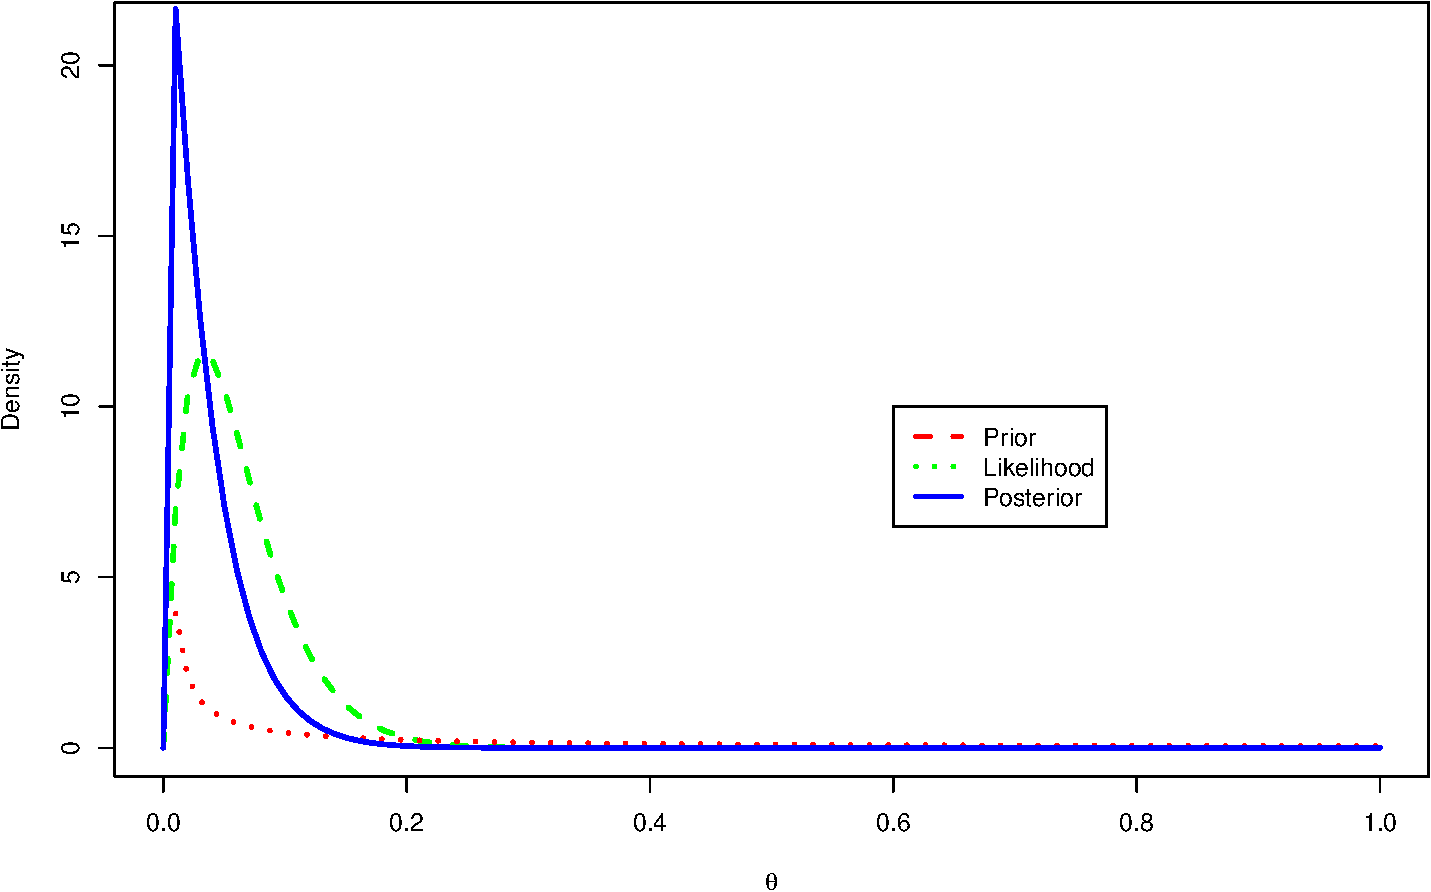
\includegraphics{02-intro-to-Bayes_files/figure-beamer/unnamed-chunk-2-1.pdf}

\end{frame}

\begin{frame}[fragile]{The loss function}
\protect\hypertarget{the-loss-function}{}

\begin{Shaded}
\begin{Highlighting}[]
\CommentTok{# compute the loss given theta and c }
\NormalTok{loss_function =}\StringTok{ }\ControlFlowTok{function}\NormalTok{(theta, c)\{}
  \ControlFlowTok{if}\NormalTok{ (c }\OperatorTok{<}\StringTok{ }\NormalTok{theta)\{}
    \KeywordTok{return}\NormalTok{(}\DecValTok{10}\OperatorTok{*}\KeywordTok{abs}\NormalTok{(theta }\OperatorTok{-}\StringTok{ }\NormalTok{c))}
\NormalTok{  \} }\ControlFlowTok{else}\NormalTok{\{}
    \KeywordTok{return}\NormalTok{(}\KeywordTok{abs}\NormalTok{(theta }\OperatorTok{-}\StringTok{ }\NormalTok{c))}
\NormalTok{  \}}
\NormalTok{\}}
\end{Highlighting}
\end{Shaded}

\end{frame}

\begin{frame}[fragile]{Posterior risk}
\protect\hypertarget{posterior-risk}{}

\begin{Shaded}
\begin{Highlighting}[]
\CommentTok{# compute the posterior risk given c }
\CommentTok{# s is the number of random draws }
\NormalTok{posterior_risk =}\StringTok{ }\ControlFlowTok{function}\NormalTok{(c, }\DataTypeTok{s =} \DecValTok{30000}\NormalTok{)\{}
  \CommentTok{# randow draws from posterior distribution}
  \CommentTok{# which is a beta with params an and bn}
\NormalTok{  theta =}\StringTok{ }\KeywordTok{rbeta}\NormalTok{(s, an, bn)}
  
  \CommentTok{# calculating values of the loss times the posterior}
\NormalTok{  loss <-}\StringTok{ }\KeywordTok{apply}\NormalTok{(}\KeywordTok{as.matrix}\NormalTok{(theta),}\DecValTok{1}\NormalTok{,loss_function,c)}
  \CommentTok{# average values from the loss function (integral)}
\NormalTok{  risk =}\StringTok{ }\KeywordTok{mean}\NormalTok{(loss)}
\NormalTok{\}}
\end{Highlighting}
\end{Shaded}

\end{frame}

\begin{frame}[fragile]{Posterior Risk (continued)}
\protect\hypertarget{posterior-risk-continued}{}

\begin{Shaded}
\begin{Highlighting}[]
\CommentTok{# a sequence of c in [0, 0.5]}
\NormalTok{c =}\StringTok{ }\KeywordTok{seq}\NormalTok{(}\DecValTok{0}\NormalTok{, }\FloatTok{0.5}\NormalTok{, }\DataTypeTok{by =} \FloatTok{0.01}\NormalTok{)}
\NormalTok{post_risk <-}\StringTok{ }\KeywordTok{apply}\NormalTok{(}\KeywordTok{as.matrix}\NormalTok{(c),}\DecValTok{1}\NormalTok{,posterior_risk)}
\KeywordTok{head}\NormalTok{(post_risk)}
\end{Highlighting}
\end{Shaded}

\begin{verbatim}
## [1] 0.33917940 0.25367603 0.18868962 0.14489894 0.11693106 0.09453471
\end{verbatim}

\end{frame}

\begin{frame}[fragile]{Posterior expected loss/posterior risk for
disease prevelance}
\protect\hypertarget{posterior-expected-lossposterior-risk-for-disease-prevelance}{}

\begin{Shaded}
\begin{Highlighting}[]
\CommentTok{# plot posterior risk against c }

\KeywordTok{pdf}\NormalTok{(}\DataTypeTok{file=}\StringTok{"posterior-risk.pdf"}\NormalTok{)}
\KeywordTok{plot}\NormalTok{(c, post_risk, }\DataTypeTok{type =} \StringTok{'l'}\NormalTok{, }\DataTypeTok{col=}\StringTok{'blue'}\NormalTok{, }
    \DataTypeTok{lwd =} \DecValTok{3}\NormalTok{, }\DataTypeTok{ylab =}\StringTok{'p(c, x)'}\NormalTok{ )}
\KeywordTok{dev.off}\NormalTok{()}
\end{Highlighting}
\end{Shaded}

\begin{verbatim}
## pdf 
##   2
\end{verbatim}

\begin{Shaded}
\begin{Highlighting}[]
\CommentTok{# minimum of posterior risk occurs at c = 0.08}
\NormalTok{(c[}\KeywordTok{which.min}\NormalTok{(post_risk)])}
\end{Highlighting}
\end{Shaded}

\begin{verbatim}
## [1] 0.08
\end{verbatim}

\end{frame}

\begin{frame}{Posterior expected loss/posterior risk for disease
prevelance}
\protect\hypertarget{posterior-expected-lossposterior-risk-for-disease-prevelance-1}{}

\begin{figure}
  \begin{center}
    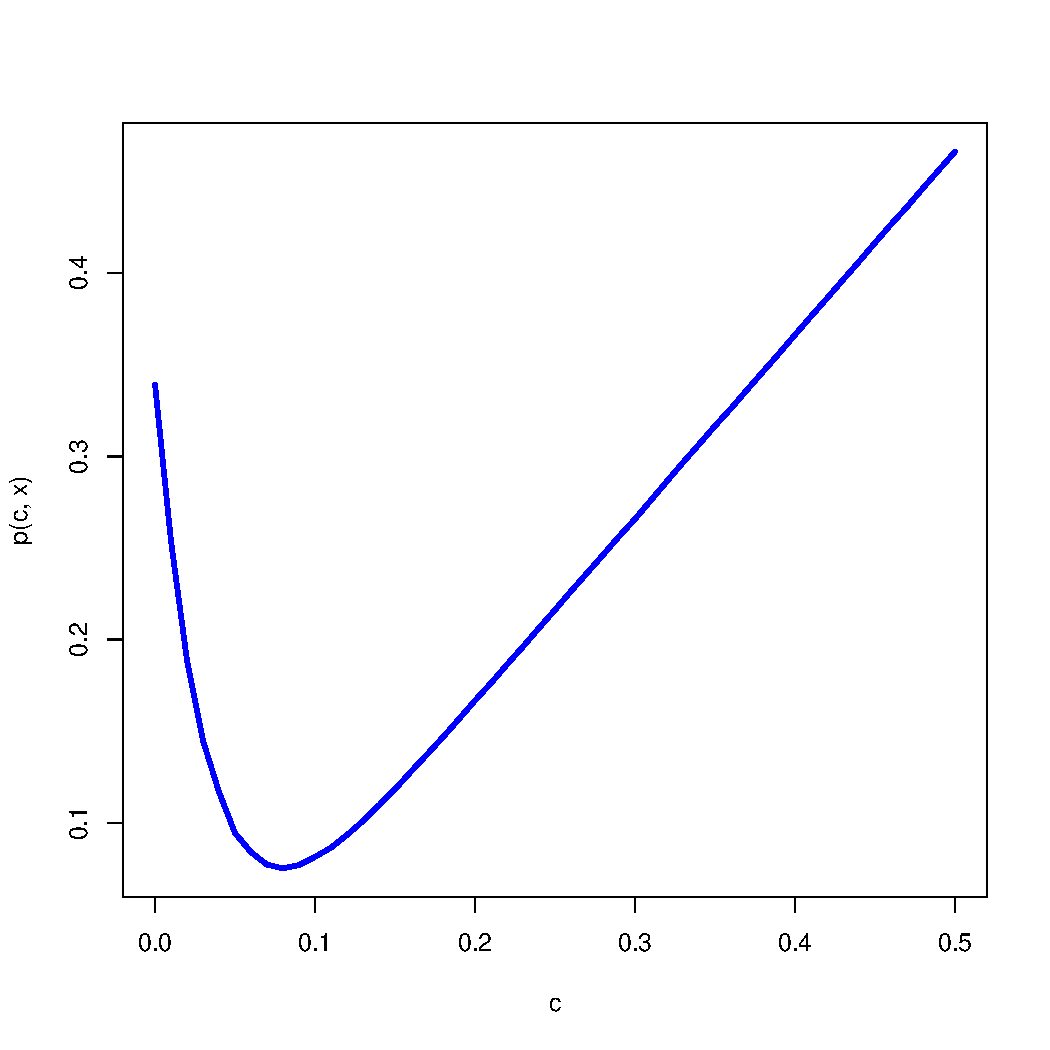
\includegraphics[width=0.6\textwidth]{figures/posterior-risk}
    % Source: Original work by R.C. Steorts
  \end{center}
  \caption{}
 \label{figure:rho}
\end{figure}

\end{frame}

\begin{frame}{Sensitivity Analysis}
\protect\hypertarget{sensitivity-analysis}{}

\textcolor{red}{Suppose now that $a = 0.05, 1, 0.05$ and $b = 1, 2, 10.$}

\textcolor{red}{If we have different prior, the posterior risk is minimized at different $c$ values. The optimal $c$ depends on not only the data, but also the prior setting.}

\end{frame}

\begin{frame}[fragile]{Posterior Risk Function (More Advanced)}
\protect\hypertarget{posterior-risk-function-more-advanced}{}

\begin{Shaded}
\begin{Highlighting}[]
\CommentTok{# compute the posterior risk given c }
\CommentTok{# s is the number of random draws }
\NormalTok{posterior_risk =}\StringTok{ }\ControlFlowTok{function}\NormalTok{(c, a_prior, b_prior, }
\NormalTok{                          sum_x, n, }\DataTypeTok{s =} \DecValTok{30000}\NormalTok{)\{}
  \CommentTok{# randow draws from beta distribution }
\NormalTok{  a_post =}\StringTok{ }\NormalTok{a_prior }\OperatorTok{+}\StringTok{ }\NormalTok{sum_x}
\NormalTok{  b_post =}\StringTok{ }\NormalTok{b_prior }\OperatorTok{+}\StringTok{ }\NormalTok{n }\OperatorTok{-}\StringTok{ }\NormalTok{sum_x}
\NormalTok{  theta =}\StringTok{ }\KeywordTok{rbeta}\NormalTok{(s, a_post, b_post)}
\NormalTok{  loss <-}\StringTok{ }\KeywordTok{apply}\NormalTok{(}\KeywordTok{as.matrix}\NormalTok{(theta),}\DecValTok{1}\NormalTok{,loss_function,c)}
  \CommentTok{# average values from the loss function}
\NormalTok{  risk =}\StringTok{ }\KeywordTok{mean}\NormalTok{(loss)}
\NormalTok{\}}
\end{Highlighting}
\end{Shaded}

\end{frame}

\begin{frame}[fragile]{Posterior Risk Function (More Advanced)}
\protect\hypertarget{posterior-risk-function-more-advanced-1}{}

\begin{Shaded}
\begin{Highlighting}[]
\CommentTok{# a sequence of c in [0, 0.5]}
\NormalTok{c =}\StringTok{ }\KeywordTok{seq}\NormalTok{(}\DecValTok{0}\NormalTok{, }\FloatTok{0.5}\NormalTok{, }\DataTypeTok{by =} \FloatTok{0.01}\NormalTok{)}
\NormalTok{post_risk <-}\StringTok{ }\KeywordTok{apply}\NormalTok{(}\KeywordTok{as.matrix}\NormalTok{(c),}\DecValTok{1}\NormalTok{,}
\NormalTok{                   posterior_risk, a, b, sum_x, n)}
\KeywordTok{head}\NormalTok{(post_risk)}
\end{Highlighting}
\end{Shaded}

\begin{verbatim}
## [1] 0.33742709 0.25432988 0.19124960 0.14450410 0.11565159 0.09530153
\end{verbatim}

\end{frame}

\begin{frame}[fragile]{Sensitivity Analysis}
\protect\hypertarget{sensitivity-analysis-1}{}

\begin{Shaded}
\begin{Highlighting}[]
\CommentTok{# set prior}
\NormalTok{as =}\StringTok{ }\KeywordTok{c}\NormalTok{(}\FloatTok{0.05}\NormalTok{, }\DecValTok{1}\NormalTok{, }\FloatTok{0.05}\NormalTok{); bs =}\StringTok{ }\KeywordTok{c}\NormalTok{(}\DecValTok{1}\NormalTok{, }\DecValTok{1}\NormalTok{, }\DecValTok{10}\NormalTok{)}
\NormalTok{post_risk =}\StringTok{ }\KeywordTok{matrix}\NormalTok{(}\OtherTok{NA}\NormalTok{, }\DecValTok{3}\NormalTok{, }\KeywordTok{length}\NormalTok{(c))}

\CommentTok{# for each pair of a and b, compute the posterior risks}
\ControlFlowTok{for}\NormalTok{ (i }\ControlFlowTok{in} \DecValTok{1}\OperatorTok{:}\DecValTok{3}\NormalTok{)\{}
\NormalTok{  a_prior =}\StringTok{ }\NormalTok{as[i]}
\NormalTok{  b_prior =}\StringTok{ }\NormalTok{bs[i]}

  \CommentTok{# using the more advanced function }
  \CommentTok{# of the posterior risk  }
\NormalTok{post_risk[i,] =}\StringTok{ }\KeywordTok{apply}\NormalTok{(}\KeywordTok{as.matrix}\NormalTok{(c), }\DecValTok{1}\NormalTok{,}
\NormalTok{                      posterior_risk, a_prior,}
\NormalTok{                      b_prior, sum_x, n)}
\NormalTok{\}}
\end{Highlighting}
\end{Shaded}

\end{frame}

\begin{frame}[fragile]{Plot}
\protect\hypertarget{plot}{}

\begin{Shaded}
\begin{Highlighting}[]
\KeywordTok{plot}\NormalTok{(c, post_risk[}\DecValTok{1}\NormalTok{,], }\DataTypeTok{type =} \StringTok{'l'}\NormalTok{, }
     \DataTypeTok{col=}\StringTok{'blue'}\NormalTok{, }\DataTypeTok{lty =} \DecValTok{1}\NormalTok{, }\DataTypeTok{yaxt =} \StringTok{"n"}\NormalTok{, }\DataTypeTok{ylab =} \StringTok{"p(c, x)"}\NormalTok{)}
\KeywordTok{par}\NormalTok{(}\DataTypeTok{new =}\NormalTok{ T)}
\KeywordTok{plot}\NormalTok{(c, post_risk[}\DecValTok{2}\NormalTok{,], }\DataTypeTok{type =} \StringTok{'l'}\NormalTok{, }
     \DataTypeTok{col=}\StringTok{'red'}\NormalTok{, }\DataTypeTok{lty =} \DecValTok{2}\NormalTok{, }\DataTypeTok{yaxt =} \StringTok{"n"}\NormalTok{, }\DataTypeTok{ylab =} \StringTok{""}\NormalTok{)}
\KeywordTok{par}\NormalTok{(}\DataTypeTok{new =}\NormalTok{ T)}
\KeywordTok{plot}\NormalTok{(c, post_risk[}\DecValTok{3}\NormalTok{,], }\DataTypeTok{type =} \StringTok{'l'}\NormalTok{, }
     \DataTypeTok{lty =} \DecValTok{3}\NormalTok{, }\DataTypeTok{yaxt =} \StringTok{"n"}\NormalTok{, }\DataTypeTok{ylab =} \StringTok{""}\NormalTok{)}
\KeywordTok{legend}\NormalTok{(}\StringTok{"bottomright"}\NormalTok{, }\DataTypeTok{lty =} \KeywordTok{c}\NormalTok{(}\DecValTok{1}\NormalTok{,}\DecValTok{2}\NormalTok{,}\DecValTok{3}\NormalTok{), }
       \DataTypeTok{col =} \KeywordTok{c}\NormalTok{(}\StringTok{"blue"}\NormalTok{, }\StringTok{"red"}\NormalTok{, }\StringTok{"black"}\NormalTok{), }
       \DataTypeTok{legend =} \KeywordTok{c}\NormalTok{(}\StringTok{"a = 0.05 b = 1"}\NormalTok{, }
                  \StringTok{"a = 1 b = 1"}\NormalTok{, }\StringTok{"a = 0.05 b = 5"}\NormalTok{))}
\end{Highlighting}
\end{Shaded}

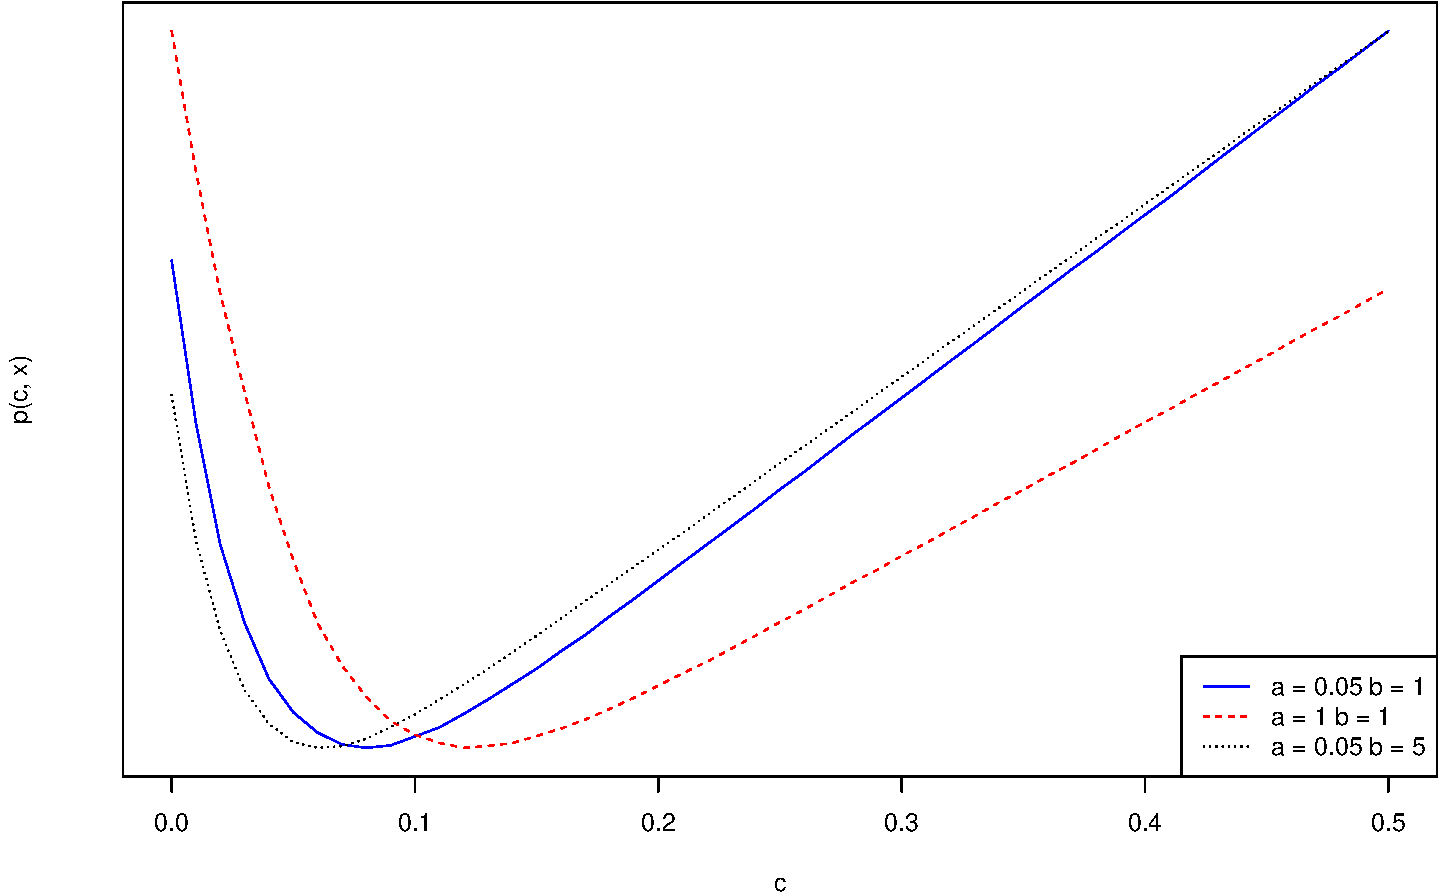
\includegraphics{02-intro-to-Bayes_files/figure-beamer/unnamed-chunk-10-1.pdf}

\end{frame}

\begin{frame}[fragile]{Optimal resources (a,b vary)}
\protect\hypertarget{optimal-resources-ab-vary}{}

\textcolor{red}{For $a = 0.05, 1, 0.05$ and $b = 1, 2, 10$ respectively,
the optimal value for c is:}

\begin{Shaded}
\begin{Highlighting}[]
\NormalTok{(c[}\KeywordTok{which.min}\NormalTok{(post_risk[}\DecValTok{1}\NormalTok{,])])}
\end{Highlighting}
\end{Shaded}

\begin{verbatim}
## [1] 0.08
\end{verbatim}

\begin{Shaded}
\begin{Highlighting}[]
\NormalTok{(c[}\KeywordTok{which.min}\NormalTok{(post_risk[}\DecValTok{2}\NormalTok{,])])}
\end{Highlighting}
\end{Shaded}

\begin{verbatim}
## [1] 0.12
\end{verbatim}

\begin{Shaded}
\begin{Highlighting}[]
\NormalTok{(c[}\KeywordTok{which.min}\NormalTok{(post_risk[}\DecValTok{3}\NormalTok{,])])}
\end{Highlighting}
\end{Shaded}

\begin{verbatim}
## [1] 0.06
\end{verbatim}

\end{frame}

\begin{frame}{Plot}
\protect\hypertarget{plot-1}{}

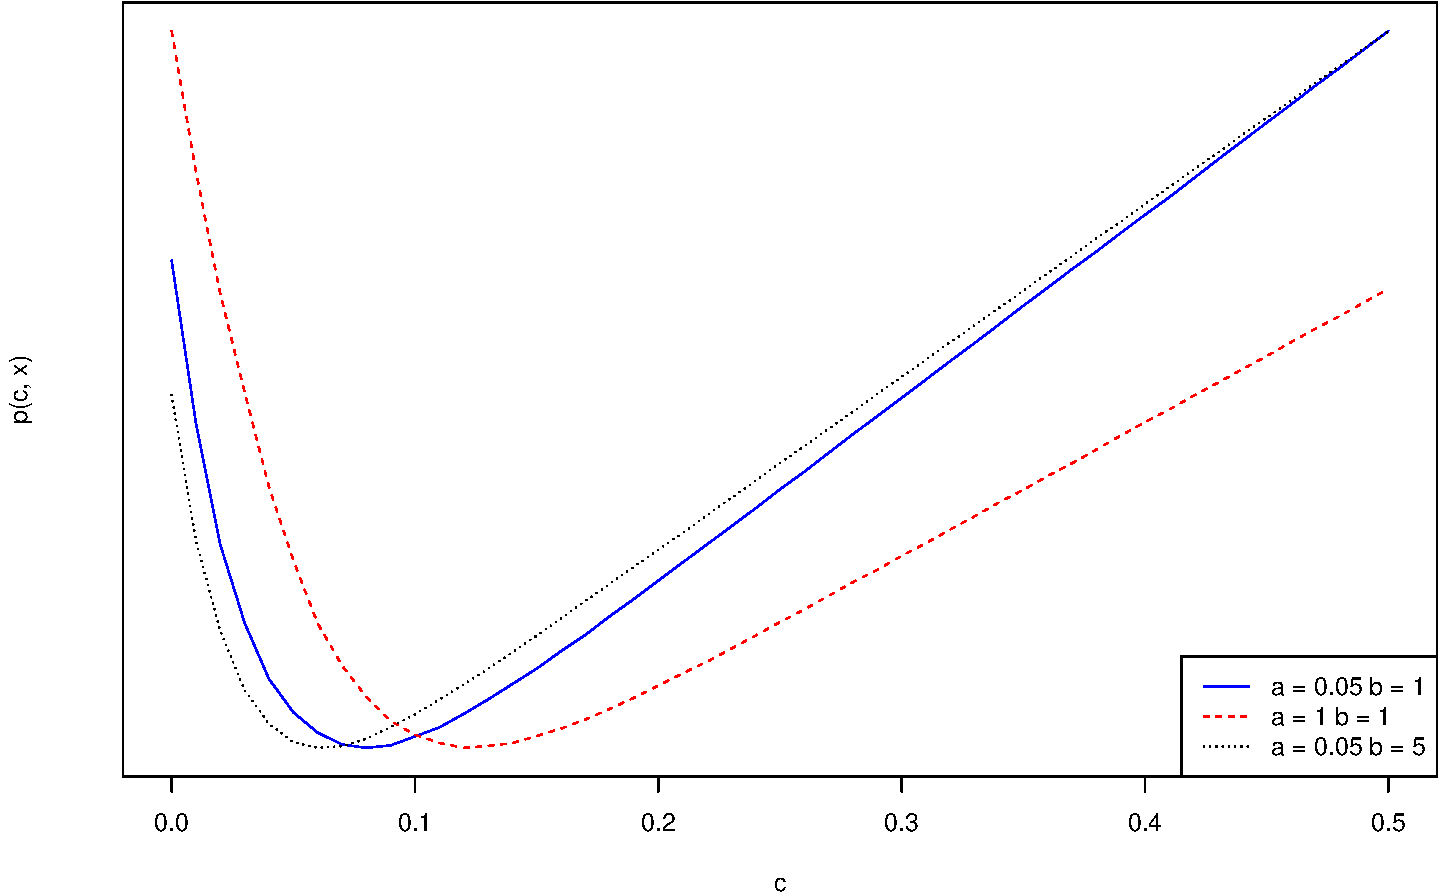
\includegraphics{02-intro-to-Bayes_files/figure-beamer/unnamed-chunk-12-1.pdf}

\end{frame}

\begin{frame}{Frequentist Risk}
\protect\hypertarget{frequentist-risk}{}

\begin{enumerate}
\tightlist
\item
  Consider a decision problem in which \(S = \btheta\).
\item
  The \term{risk} (or \term{frequentist risk}) associated with a
  decision procedure \(\delta\) is
  \[ R(\theta,\delta) = \E\big(\ell(\btheta,\delta(X))\mid\btheta =\theta\big),\]
  where \(X\) has distribution \(p(x|\btheta)\). In other words,
  \[ R(\theta,\delta) = \int \ell(\theta,\delta(x))\,p(x|\theta)\,dx\]
  if \(X\) is continuous, while the integral is replaced with a sum if
  \(X\) is discrete.
\end{enumerate}

\end{frame}

\begin{frame}{The integrated risk}
\protect\hypertarget{the-integrated-risk}{}

The \term{integrated risk} associated with \(\delta(X)\) is
\begin{align}
r(\delta) &= \E(\ell(\btheta,\delta(X)) = \int R(\theta,\delta)\,p(\theta)\,d\theta \\
&= \int \int \ell(\theta,\delta(x))\,p(x|\theta)p(\theta)\,dx \,d\theta
\end{align}

\end{frame}

\begin{frame}{Example: Resource allocation, revisited}
\protect\hypertarget{example-resource-allocation-revisited}{}

\begin{enumerate}
\tightlist
\item
  The frequentist risk provides a useful way to compare decision
  procedures in a prior-free way.
\item
  In addition to the Bayes procedure or Bayes rule that we have
  considered earlier in the lecture, consider two other potential
  optimal decision rules: choosing \(c = \bar x\) (sample mean) or
  \(c=0.1\)
  (constant).\footnote{Recall: The Bayes rule minimizes the posterior risk with respect to the parameter of interest.}
\item
  \textcolor{red}{Remark: both the frequentist rules are looking an optimal estimator in a prior free way. (There are many other examples, but we'll just look at two simple cases.)}
\end{enumerate}

\end{frame}

\begin{frame}{Example: Resource allocation, revisited}
\protect\hypertarget{example-resource-allocation-revisited-1}{}

\begin{enumerate}
\setcounter{enumi}{2}
\tightlist
\item
  Figure \ref{figure:procedures} shows each procedure as a function of
  \(\sum x_i\), the observed number of diseased cases. For the prior we
  have chosen, the Bayes procedure always picks \(c\) to be a little
  bigger than \(\bar x\).
\end{enumerate}

\begin{figure}
  \begin{center}
    \includegraphics[width=0.85\textwidth]{figures/procedures.png}
    % Source: Original work by J. W. Miller.
  \end{center}
  \caption{Resources allocated $c$, as a function of the number of diseased individuals observed, $\sum x_i$, for the three different procedures.}
  \label{figure:procedures}
\end{figure}

\end{frame}

\begin{frame}{Example: Resource allocation, revisited}
\protect\hypertarget{example-resource-allocation-revisited-2}{}

\begin{enumerate}
\setcounter{enumi}{3}
\tightlist
\item
  Figure \ref{figure:risk} shows the risk \(R(\theta,\delta)\) as a
  function of \(\theta\) for each procedure. Smaller risk is better.
  (Recall that for each \(\theta\), the risk is the expected loss,
  averaging over all possible data sets. The observed data doesn't
  factor into it at all.)
\end{enumerate}

\begin{figure}
  \begin{center}
    \includegraphics[width=0.85\textwidth]{figures/risk.png}
    % Source: Original work by J. W. Miller.
  \end{center}
  \caption{Risk functions for the three different procedures.}
  \label{figure:risk}
\end{figure}

\end{frame}

\begin{frame}{Example: Resource allocation, revisited}
\protect\hypertarget{example-resource-allocation-revisited-3}{}

\begin{enumerate}
\setcounter{enumi}{4}
\tightlist
\item
  The constant procedure is fantastic when \(\theta\) is near \(0.1\),
  but gets very bad very quickly for larger \(\theta\). The Bayes
  procedure is better than the sample mean for nearly all \(\theta\)'s.
  These curves reflect the usual situation---some procedures will work
  better for certain \(\theta\)'s and some will work better for others.
\item
  A decision procedure which is \term{inadmissible} is one that is
  dominated everywhere. That is, \(\delta\) is
  \term{\textcolor{red}{admissible}} if there is no \(\delta'\) such
  that \[R(\theta,\delta')\leq R(\theta,\delta)\] for all \(\theta\) and
  \(R(\theta,\delta')< R(\theta,\delta)\) for at least one \(\theta\).
  \textcolor{red}{A decision rule is admissible so long as it is not being dominated everywhere.}\\
\item
  Bayes procedures are admissible under very general conditions.
\item
  Admissibility is nice to have, but it doesn't mean a procedure is
  necessarily good. Silly procedures can still be admissible---e.g., in
  this example, the constant procedure \(c = 0.1\) is admissible too!
\end{enumerate}

\end{frame}

\begin{frame}{Takeaways}
\protect\hypertarget{takeaways}{}

\begin{itemize}
\item
  In understanding an optimal decision rule, we first must have a
  parameter of interest (\(\theta\)) and define an optimal estimator
  (\(\delta(X)\) or \(\hat{\theta}\)).
\item
  There are many ways to define a loss function. A few that we talked
  about were the 0-1, quadratic, and absolute value loss.
\item
  Next, we define several ways of finding an optimal decision rule.
  There were three that we considered. We considered minimizing the
  posterior risk (Bayes rule), the risk (frequentist risk), or the
  integrated risk.
\item
  Finally, we defined admissible/inadmissible rules.
\end{itemize}

\end{frame}

\begin{frame}{Detailed Takeways for Exam}
\protect\hypertarget{detailed-takeways-for-exam}{}

\begin{itemize}
\tightlist
\item
  \(\hat{\theta}\) is an estimator of \(\theta\)
\item
  Loss function \(L(\theta, \hat{\theta})\)
\item
  Examples of loss functions
\item
  The difference between an action and an estimator
\item
  Posterior risk
\item
  Decision procedure
\item
  Bayes rule (or Bayes estimator)
\item
  How to derive the Bayes estimator
\item
  What is the Bayes estimator under squared error loss?
\item
  What is the Bayes estimator under weighted squared error loss?
\item
  When you find the Bayes estimator, what condition do you always need
  to check?
\end{itemize}

\end{frame}

\begin{frame}{Detailed Takeways for Exam (Continued)}
\protect\hypertarget{detailed-takeways-for-exam-continued}{}

\begin{itemize}
\tightlist
\item
  How to approach decision theory problems such as the resource
  allocation problem, where you're given the set up and then you must
  given the model and the loss function and back up the rational here.
\item
  How to solve for the Bayes estimator for an applied problem such as
  the resource allocation problem, where the Bayes estimator is NOT in a
  closed form solution.
\item
  How to conduct a sensitivity analysis for a posterior analysis and
  report your findings.
\item
  The frequentist risk and why it's used.
\item
  The integrated risk and why it's used.
\item
  Admissibility and how to determine if an estimator is admissible or
  inadmissible.
\end{itemize}

\end{frame}

\begin{frame}{Module 2 Derivations}
\protect\hypertarget{module-2-derivations}{}

Module 2 Derivations can be found below:

\url{https://github.com/resteorts/modern-bayes/tree/master/lecturesModernBayes20/lecture-2/02-class-notes}

\end{frame}

\end{document}
